
\documentclass[journal,12pt,twocolumn]{IEEEtran}
%
\usepackage{setspace}
\usepackage{gensymb}
%\doublespacing
\singlespacing

%\usepackage{graphicx}
%\usepackage{amssymb}
%\usepackage{relsize}
\usepackage[cmex10]{amsmath}
%\usepackage{amsthm}
%\interdisplaylinepenalty=2500
%\savesymbol{iint}
%\usepackage{txfonts}
%\restoresymbol{TXF}{iint}
%\usepackage{wasysym}
\usepackage{amsthm}
%\usepackage{iithtlc}
\usepackage{mathrsfs}
\usepackage{txfonts}
\usepackage{stfloats}
\usepackage{bm}
\usepackage{cite}
\usepackage{cases}
\usepackage{subfig}
%\usepackage{xtab}
\usepackage{longtable}
\usepackage{multirow}
%\usepackage{algorithm}
%\usepackage{algpseudocode}
\usepackage{enumitem}
\usepackage{mathtools}
\usepackage{tikz}
\usepackage[american]{circuitikz}
\usepackage{verbatim}
\usepackage{tfrupee}
\usepackage[breaklinks=true]{hyperref}
%\usepackage{stmaryrd}
\usepackage{tkz-euclide} % loads  TikZ and tkz-base
\usetkzobj{all}
\usetikzlibrary{decorations.markings}
\usetikzlibrary{shapes.geometric}
\newif\iflabrev
\usepackage{listings}
    \usepackage{color}                                            %%
    \usepackage{array}                                            %%
    \usepackage{longtable}                                        %%
    \usepackage{calc}                                             %%
    \usepackage{multirow}                                         %%
    \usepackage{hhline}                                           %%
    \usepackage{ifthen}                                           %%
  %optionally (for landscape tables embedded in another document): %%
    \usepackage{lscape}     
\usepackage{multicol}
\usepackage{chngcntr}
%\usepackage{enumerate}

%\usepackage{wasysym}
%\newcounter{MYtempeqncnt}
\DeclareMathOperator*{\Res}{Res}
%\renewcommand{\baselinestretch}{2}
\renewcommand\thesection{\arabic{section}}
\renewcommand\thesubsection{\thesection.\arabic{subsection}}
\renewcommand\thesubsubsection{\thesubsection.\arabic{subsubsection}}

\renewcommand\thesectiondis{\arabic{section}}
\renewcommand\thesubsectiondis{\thesectiondis.\arabic{subsection}}
\renewcommand\thesubsubsectiondis{\thesubsectiondis.\arabic{subsubsection}}

% correct bad hyphenation here
\hyphenation{op-tical net-works semi-conduc-tor}
\def\inputGnumericTable{}                                 %%

\lstset{
%language=C,
frame=single, 
breaklines=true,
columns=fullflexible
}
%\lstset{
%language=tex,
%frame=single, 
%breaklines=true
%}

\begin{document}
%


\newtheorem{theorem}{Theorem}[section]
\newtheorem{problem}{Problem}
\newtheorem{proposition}{Proposition}[section]
\newtheorem{lemma}{Lemma}[section]
\newtheorem{corollary}[theorem]{Corollary}
\newtheorem{example}{Example}[section]
\newtheorem{definition}[problem]{Definition}
%\newtheorem{thm}{Theorem}[section] 
%\newtheorem{defn}[thm]{Definition}
%\newtheorem{algorithm}{Algorithm}[section]
%\newtheorem{cor}{Corollary}
\newcommand{\BEQA}{\begin{eqnarray}}
\newcommand{\EEQA}{\end{eqnarray}}
\newcommand{\define}{\stackrel{\triangle}{=}}
\bibliographystyle{IEEEtran}
%\bibliographystyle{ieeetr}
\providecommand{\mbf}{\mathbf}
\providecommand{\pr}[1]{\ensuremath{\Pr\left(#1\right)}}
\providecommand{\qfunc}[1]{\ensuremath{Q\left(#1\right)}}
\providecommand{\sbrak}[1]{\ensuremath{{}\left[#1\right]}}
\providecommand{\lsbrak}[1]{\ensuremath{{}\left[#1\right.}}
\providecommand{\rsbrak}[1]{\ensuremath{{}\left.#1\right]}}
\providecommand{\brak}[1]{\ensuremath{\left(#1\right)}}
\providecommand{\lbrak}[1]{\ensuremath{\left(#1\right.}}
\providecommand{\rbrak}[1]{\ensuremath{\left.#1\right)}}
\providecommand{\cbrak}[1]{\ensuremath{\left\{#1\right\}}}
\providecommand{\lcbrak}[1]{\ensuremath{\left\{#1\right.}}
\providecommand{\rcbrak}[1]{\ensuremath{\left.#1\right\}}}
\theoremstyle{remark}
\newtheorem{rem}{Remark}
\newcommand{\sgn}{\mathop{\mathrm{sgn}}}
\DeclarePairedDelimiter\abs{\lvert}{\rvert}
% \providecommand{\res}[1]{\Res\displaylimits_{#1}} 
% \providecommand{\norm}[1]{\left\lVert#1\right\rVert}
% %\providecommand{\norm}[1]{\lVert#1\rVert}
% \providecommand{\mtx}[1]{\mathbf{#1}}
% \providecommand{\mean}[1]{E\left[ #1 \right]}
\providecommand{\fourier}{\overset{\mathcal{F}}{ \rightleftharpoons}}
%\providecommand{\hilbert}{\overset{\mathcal{H}}{ \rightleftharpoons}}
\providecommand{\system}{\overset{\mathcal{H}}{ \longleftrightarrow}}
	%\newcommand{\solution}[2]{\textbf{Solution:}{#1}}
\newcommand{\solution}{\noindent \textbf{Solution: }}
\newcommand{\cosec}{\,\text{cosec}\,}
\providecommand{\dec}[2]{\ensuremath{\overset{#1}{\underset{#2}{\gtrless}}}}
\newcommand{\myvec}[1]{\ensuremath{\begin{pmatrix}#1\end{pmatrix}}}
\newcommand{\mydet}[1]{\ensuremath{\begin{vmatrix}#1\end{vmatrix}}}
%\numberwithin{equation}{section}
\numberwithin{equation}{subsection}
%\numberwithin{problem}{section}
%\numberwithin{definition}{section}
\makeatletter
\@addtoreset{figure}{problem}
\makeatother
\let\StandardTheFigure\thefigure
\let\vec\mathbf
%\renewcommand{\thefigure}{\theproblem.\arabic{figure}}
\renewcommand{\thefigure}{\theproblem}
%\setlist[enumerate,1]{before=\renewcommand\theequation{\theenumi.\arabic{equation}}
%\counterwithin{equation}{enumi}
%\renewcommand{\theequation}{\arabic{subsection}.\arabic{equation}}
\def\putbox#1#2#3{\makebox[0in][l]{\makebox[#1][l]{}\raisebox{\baselineskip}[0in][0in]{\raisebox{#2}[0in][0in]{#3}}}}
     \def\rightbox#1{\makebox[0in][r]{#1}}
     \def\centbox#1{\makebox[0in]{#1}}
     \def\topbox#1{\raisebox{-\baselineskip}[0in][0in]{#1}}
     \def\midbox#1{\raisebox{-0.5\baselineskip}[0in][0in]{#1}}
\vspace{3cm}
\title{
%	\logo{
Feedback and Poles
%	}
}
\author{ Piyush Kumar Uttam$^{*}$% <-this % stops a space
	\thanks{*The author is with the Department
		of Electrical Engineering, Indian Institute of Technology, Hyderabad
		502285 India e-mail:  gadepall@iith.ac.in. All content in this manual is released under GNU GPL.  Free and open source.}
	
}	
%\title{
%	\logo{Matrix Analysis through Octave}{\begin{center}\includegraphics[scale=.24]{tlc}\end{center}}{}{HAMDSP}
%}
% paper title
% can use linebreaks \\ within to get better formatting as desired
%\title{Matrix Analysis through Octave}
%
%
% author names and IEEE memberships
% note positions of commas and nonbreaking spaces ( ~ ) LaTeX will not break
% a structure at a ~ so this keeps an author's name from being broken across
% two lines.
% use \thanks{} to gain access to the first footnote area
% a separate \thanks must be used for each paragraph as LaTeX2e's \thanks
% was not built to handle multiple paragraphs
%
%\author{<-this % stops a space
%\thanks{}}
%}
% note the % following the last \IEEEmembership and also \thanks - 
% these prevent an unwanted space from occurring between the last author name
% and the end of the author line. i.e., if you had this:
% 
% \author{....lastname \thanks{...} \thanks{...} }
%                     ^------------^------------^----Do not want these spaces!
%
% a space would be appended to the last name and could cause every name on that
% line to be shifted left slightly. This is one of those "LaTeX things". For
% instance, "\textbf{A} \textbf{B}" will typeset as "A B" not "AB". To get
% "AB" then you have to do: "\textbf{A}\textbf{B}"
% \thanks is no different in this regard, so shield the last } of each \thanks
% that ends a line with a % and do not let a space in before the next \thanks.
% Spaces after \IEEEmembership other than the last one are OK (and needed) as
% you are supposed to have spaces between the names. For what it is worth,
% this is a minor point as most people would not even notice if the said evil
% space somehow managed to creep in.
% The paper headers
%\markboth{Journal of \LaTeX\ Class Files,~Vol.~6, No.~1, January~2007}%
%{Shell \MakeLowercase{\textit{et al.}}: Bare Demo of IEEEtran.cls for Journals}
% The only time the second header will appear is for the odd numbered pages
% after the title page when using the twoside option.
% 
% *** Note that you probably will NOT want to include the author's ***
% *** name in the headers of peer review papers.                   ***
% You can use \ifCLASSOPTIONpeerreview for conditional compilation here if
% you desire.
% If you want to put a publisher's ID mark on the page you can do it like
% this:
%\IEEEpubid{0000--0000/00\$00.00~\copyright~2007 IEEE}
% Remember, if you use this you must call \IEEEpubidadjcol in the second
% column for its text to clear the IEEEpubid mark.
% make the title area
\maketitle
%\newpage
%\tableofcontents
\bigskip
\renewcommand{\thefigure}{\theenumi}
\renewcommand{\thetable}{\theenumi}
%\renewcommand{\theequation}{\theenumi}
%\begin{abstract}
%%\boldmath
%In this letter, an algorithm for evaluating the exact analytical bit error rate  (BER)  for the piecewise linear (PL) combiner for  multiple relays is presented. Previous results were available only for upto three relays. The algorithm is unique in the sense that  the actual mathematical expressions, that are prohibitively large, need not be explicitly obtained. The diversity gain due to multiple relays is shown through plots of the analytical BER, well supported by simulations. 
%
%\end{abstract}
% IEEEtran.cls defaults to using nonbold math in the Abstract.
% This preserves the distinction between vectors and scalars. However,
% if the journal you are submitting to favors bold math in the abstract,
% then you can use LaTeX's standard command \boldmath at the very start
% of the abstract to achieve this. Many IEEE journals frown on math
% in the abstract anyway.
% Note that keywords are not normally used for peerreview papers.
%\begin{IEEEkeywords}
%Cooperative diversity, decode and forward, piecewise linear
%\end{IEEEkeywords}
% For peer review papers, you can put extra information on the cover
% page as needed:
% \ifCLASSOPTIONpeerreview
% \begin{center} \bfseries EDICS Category: 3-BBND \end{center}
% \fi
%
% For peerreview papers, this IEEEtran command inserts a page break and
% creates the second title. It will be ignored for other modes.
%\IEEEpeerreviewmaketitle

%\begin{abstract}
%This manual is an introduction to control systems based on GATE problems.Links to sample Python codes are available in the text.  
%\end{abstract}
%Download python codes using 
%\begin{lstlisting}
%svn co https://github.com/gadepall/school/trunk/control/codes
%\end{lstlisting}
%\section{Feedback Circuits}
An amplifier having a low-frequency gain of 1000 and poles at $10^4$ Hz and $10^5$ Hz is operated in a closed negative-feedback loop with a frequency-independent $H$.  
\begin{enumerate}[label=\alph*.]
\item  For what value of H do the closed-loop poles become coincident? At what frequency?\\
\item  What is the low-frequency gain corresponding to the situation in (a)? What is the value of the closed-loop gain at the frequency of the coincident poles?\\
\item  What is the value of Q corresponding to the situation in(a)?\\
\item If H is increased by a factor of 10, what are the new pole locations? What is the corresponding pole Q?
\end{enumerate}
%\begin{enumerate}[label=\thesubsection.\arabic*.,ref=\thesubsection.\theenumi]
\begin{enumerate}[label=\arabic*.,ref=\theenumi]
\numberwithin{equation}{enumi}

\item Find $G(s)$
\\
\solution Given, low frequency Gain and two poles.Therefore,G(s) can be written as..,
\begin{align}
  G(s) &= \frac{G_0}{\brak{1+\frac{s}{p_{1}}}\brak{1+\frac{s}{p_{2}}}} 
\label{eq:ee18btech11036_open_loop_gain} 
\end{align}
where the parameters are tabulated in Table \ref{table:ee18btech11036_ Input_Table}

\begin{table}[!ht]
\centering

%%%%%%%%%%%%%%%%%%%%%%%%%%%%%%%%%%%%%%%%%%%%%%%%%%%%%%%%%%%%%%%%%%%%%%
%%                                                                  %%
%%  This is the header of a LaTeX2e file exported from Gnumeric.    %%
%%                                                                  %%
%%  This file can be compiled as it stands or included in another   %%
%%  LaTeX document. The table is based on the longtable package so  %%
%%  the longtable options (headers, footers...) can be set in the   %%
%%  preamble section below (see PRAMBLE).                           %%
%%                                                                  %%
%%  To include the file in another, the following two lines must be %%
%%  in the including file:                                          %%
%%        \def\inputGnumericTable{}                                 %%
%%  at the beginning of the file and:                               %%
%%        \input{name-of-this-file.tex}                             %%
%%  where the table is to be placed. Note also that the including   %%
%%  file must use the following packages for the table to be        %%
%%  rendered correctly:                                             %%
%%    \usepackage[latin1]{inputenc}                                 %%
%%    \usepackage{color}                                            %%
%%    \usepackage{array}                                            %%
%%    \usepackage{longtable}                                        %%
%%    \usepackage{calc}                                             %%
%%    \usepackage{multirow}                                         %%
%%    \usepackage{hhline}                                           %%
%%    \usepackage{ifthen}                                           %%
%%  optionally (for landscape tables embedded in another document): %%
%%    \usepackage{lscape}                                           %%
%%                                                                  %%
%%%%%%%%%%%%%%%%%%%%%%%%%%%%%%%%%%%%%%%%%%%%%%%%%%%%%%%%%%%%%%%%%%%%%%



%%  This section checks if we are begin input into another file or  %%
%%  the file will be compiled alone. First use a macro taken from   %%
%%  the TeXbook ex 7.7 (suggestion of Han-Wen Nienhuys).            %%
\def\ifundefined#1{\expandafter\ifx\csname#1\endcsname\relax}


%%  Check for the \def token for inputed files. If it is not        %%
%%  defined, the file will be processed as a standalone and the     %%
%%  preamble will be used.                                          %%
\ifundefined{inputGnumericTable}

%%  We must be able to close or not the document at the end.        %%
	\def\gnumericTableEnd{\end{document}}


%%%%%%%%%%%%%%%%%%%%%%%%%%%%%%%%%%%%%%%%%%%%%%%%%%%%%%%%%%%%%%%%%%%%%%
%%                                                                  %%
%%  This is the PREAMBLE. Change these values to get the right      %%
%%  paper size and other niceties.                                  %%
%%                                                                  %%
%%%%%%%%%%%%%%%%%%%%%%%%%%%%%%%%%%%%%%%%%%%%%%%%%%%%%%%%%%%%%%%%%%%%%%

	\documentclass[12pt%
			  %,landscape%
                    ]{report}
       \usepackage[latin1]{inputenc}
       \usepackage{fullpage}
       \usepackage{color}
       \usepackage{array}
       \usepackage{longtable}
       \usepackage{calc}
       \usepackage{multirow}
       \usepackage{hhline}
       \usepackage{ifthen}



%%  End of the preamble for the standalone. The next section is for %%
%%  documents which are included into other LaTeX2e files.          %%
\else

%%  We are not a stand alone document. For a regular table, we will %%
%%  have no preamble and only define the closing to mean nothing.   %%
    \def\gnumericTableEnd{}

%%  If we want landscape mode in an embedded document, comment out  %%
%%  the line above and uncomment the two below. The table will      %%
%%  begin on a new page and run in landscape mode.                  %%
%       \def\gnumericTableEnd{\end{landscape}}
%       \begin{landscape}


%%  End of the else clause for this file being \input.              %%
\fi

%%%%%%%%%%%%%%%%%%%%%%%%%%%%%%%%%%%%%%%%%%%%%%%%%%%%%%%%%%%%%%%%%%%%%%
%%                                                                  %%
%%  The rest is the gnumeric table, except for the closing          %%
%%  statement. Changes below will alter the table's appearance.     %%
%%                                                                  %%
%%%%%%%%%%%%%%%%%%%%%%%%%%%%%%%%%%%%%%%%%%%%%%%%%%%%%%%%%%%%%%%%%%%%%%

\providecommand{\gnumericmathit}[1]{#1} 
%%  Uncomment the next line if you would like your numbers to be in %%
%%  italics if they are italizised in the gnumeric table.           %%
%\renewcommand{\gnumericmathit}[1]{\mathit{#1}}
\providecommand{\gnumericPB}[1]%
{\let\gnumericTemp=\\#1\let\\=\gnumericTemp\hspace{0pt}}
 \ifundefined{gnumericTableWidthDefined}
        \newlength{\gnumericTableWidth}
        \newlength{\gnumericTableWidthComplete}
        \newlength{\gnumericMultiRowLength}
        \global\def\gnumericTableWidthDefined{}
 \fi
%% The following setting protects this code from babel shorthands.  %%
 \ifthenelse{\isundefined{\languageshorthands}}{}{\languageshorthands{english}}
%%  The default table format retains the relative column widths of  %%
%%  gnumeric. They can easily be changed to c, r or l. In that case %%
%%  you may want to comment out the next line and uncomment the one %%
%%  thereafter                                                      %%
\providecommand\gnumbox{\makebox[0pt]}
%%\providecommand\gnumbox[1][]{\makebox}

%% to adjust positions in multirow situations                       %%
\setlength{\bigstrutjot}{\jot}
\setlength{\extrarowheight}{\doublerulesep}

%%  The \setlongtables command keeps column widths the same across  %%
%%  pages. Simply comment out next line for varying column widths.  %%
\setlongtables

\setlength\gnumericTableWidth{%
	53pt+%
	93pt+%
0pt}
\def\gumericNumCols{2}
\setlength\gnumericTableWidthComplete{\gnumericTableWidth+%
         \tabcolsep*\gumericNumCols*2+\arrayrulewidth*\gumericNumCols}
\ifthenelse{\lengthtest{\gnumericTableWidthComplete > \linewidth}}%
         {\def\gnumericScale{\ratio{\linewidth-%
                        \tabcolsep*\gumericNumCols*2-%
                        \arrayrulewidth*\gumericNumCols}%
{\gnumericTableWidth}}}%
{\def\gnumericScale{1}}

%%%%%%%%%%%%%%%%%%%%%%%%%%%%%%%%%%%%%%%%%%%%%%%%%%%%%%%%%%%%%%%%%%%%%%
%%                                                                  %%
%% The following are the widths of the various columns. We are      %%
%% defining them here because then they are easier to change.       %%
%% Depending on the cell formats we may use them more than once.    %%
%%                                                                  %%
%%%%%%%%%%%%%%%%%%%%%%%%%%%%%%%%%%%%%%%%%%%%%%%%%%%%%%%%%%%%%%%%%%%%%%

\ifthenelse{\isundefined{\gnumericColA}}{\newlength{\gnumericColA}}{}\settowidth{\gnumericColA}{\begin{tabular}{@{}p{110pt*\gnumericScale}@{}}x\end{tabular}}
\ifthenelse{\isundefined{\gnumericColB}}{\newlength{\gnumericColB}}{}\settowidth{\gnumericColB}{\begin{tabular}{@{}p{30pt*\gnumericScale}@{}}x\end{tabular}}

\begin{tabular}[c]{%
	b{\gnumericColA}%
	b{\gnumericColB}%
	}

%%%%%%%%%%%%%%%%%%%%%%%%%%%%%%%%%%%%%%%%%%%%%%%%%%%%%%%%%%%%%%%%%%%%%%
%%  The longtable options. (Caption, headers... see Goosens, p.124) %%
%	\caption{The Table Caption.}             \\	%
% \hline	% Across the top of the table.
%%  The rest of these options are table rows which are placed on    %%
%%  the first, last or every page. Use \multicolumn if you want.    %%

%%  Header for the first page.                                      %%
%	\multicolumn{2}{c}{The First Header} \\ \hline 
%	\multicolumn{1}{c}{colTag}	%Column 1
%	&\multicolumn{1}{c}{colTag}	\\ \hline %Last column
%	\endfirsthead

%%  The running header definition.                                  %%
%	\hline
%	\multicolumn{2}{l}{\ldots\small\slshape continued} \\ \hline
%	\multicolumn{1}{c}{colTag}	%Column 1
%	&\multicolumn{1}{c}{colTag}	\\ \hline %Last column
%	\endhead

%%  The running footer definition.                                  %%
%	\hline
%	\multicolumn{2}{r}{\small\slshape continued\ldots} \\
%	\endfoot

%%  The ending footer definition.                                   %%
%	\multicolumn{2}{c}{That's all folks} \\ \hline 
%	\endlastfoot
%%%%%%%%%%%%%%%%%%%%%%%%%%%%%%%%%%%%%%%%%%%%%%%%%%%%%%%%%%%%%%%%%%%%%%

\hhline{|-|-}
	 \multicolumn{1}{|p{\gnumericColA}|}%
	{\gnumericPB{\centering}\gnumbox{\textbf{Parameter}}}
	&\multicolumn{1}{p{\gnumericColB}|}%
	{\gnumericPB{\centering}\gnumbox{\textbf{Value}}}
\\
\hhline{|-|-}
	 \multicolumn{1}{|p{\gnumericColA}|}%
	{\gnumericPB{\centering}\gnumbox{\text{Low Frequency Gain}}}
	&\multicolumn{1}{p{\gnumericColB}|}%
	{\gnumericPB{\centering}\gnumbox{\text{1000}}}
\\
\hhline{|-|-}
	 \multicolumn{1}{|p{\gnumericColA}|}%
	{\gnumericPB{\centering}\gnumbox{\text{Pole 1 (p1)}}}
	&\multicolumn{1}{p{\gnumericColB}|}%
	{\gnumericPB{\centering}\gnumbox{\text{$10^4$ Hz}}}
\\
\hhline{|-|-}
	 \multicolumn{1}{|p{\gnumericColA}|}%
	{\gnumericPB{\centering}\gnumbox{\text{Pole 2 (p2)}}}
	&\multicolumn{1}{p{\gnumericColB}|}%
	{\gnumericPB{\centering}\gnumbox{\text{$10^5$ Hz}}}
\\


\hhline{|-|-|}
\end{tabular}

\ifthenelse{\isundefined{\languageshorthands}}{}{\languageshorthands{\languagename}}
\gnumericTableEnd

\caption{}
\label{table:ee18btech11036_ Input_Table}
\end{table}
%where the parameters are listed in 
%,-p1 and -p2 are poles of G(s).
%Parameters given are shown in Table.\ref{table:ee18btech11036_ Input_Table}:1
%\begin{align}
%    G_0 &= 1000\\
%\text{Therefore.,} G(s)&= \frac{1000}{\brak{1+\frac{s}{p_{1}}}\brak{1+\frac{s}{p_{2}}}}  
%\end{align}
%Where $p_1$ and $p_2$ are 
%\begin{align}
%    p_1 &= 2\pi10^4 rad/sec\\
%    p_2 &= 2\pi10^5 rad/sec
%    \label{eq:ee18btech11036_p_values}
%\end{align}
%Now, we connect the system in a negative feedback of feedback factor H.
%We know that the closed loop gain of a negative feedback system is.,

%------------------------------
\item For what value of H do the closed-loop poles become coincident? At what frequency?\\
\solution The closed loop transfer function is
\begin{align}
\label{eq:ee18btech11036_transfer_function}
    T(s) &= \frac{G(s)}{1+G(s)H} 
%\\
% &= \frac{\frac{G_0}{\brak{1+\frac{s}{p_{1}}}\brak{1+\frac{s}{p_{2}}}}}{1+\frac{HG_0}{\brak{1+\frac{s}{p_{1}}}\brak{1+\frac{s}{p_{2}}}}}\\
%\end{align}
%\begin{align}
%    T(s) &= \frac{G_0}{\brak{1+\frac{s}{p_1}}\brak{1+\frac{s}{p_2}} + HG_0}\\
\\
    T(s) &= \frac{G_0}{\frac{s^2}{p_1p_2} + \brak{\frac{1}{p_1}+\frac{1}{p_2}}s + HG_0+1}
    \label{eq:ee18btech11036_closed_loop}
\end{align}
upon substituting from \eqref{eq:ee18btech11036_open_loop_gain}  and simplifying.  
%
For     \eqref{eq:ee18btech11036_closed_loop} to have equal roots,

%For this equation to have equal and repetitive roots, D=0
%\begin{align}
%    b^2-4ac=0
%    \label{eq:ee18btech11036_ce}
%\end{align}

\begin{align}
    \brak{\frac{1}{p_1}+\frac{1}{p_2}}^2&= \frac{4}{p_1p_2}\brak{G_0H+1}
    \label{eq:ee18btech11036_h}
%\end{align}
\\
%\begin{align}
\implies     H &= \frac{\brak{p_1-p_2}^2}{4G_0p_1p_2}
    \label{eq:ee18btech11036_h_final}
%\end{align}
%Value of H on plugging in values:
%\begin{align}
\\
    H &= 2.025 \times 10^{-3}
    \label{eq:ee18btech11036_h_value}
\end{align}
%Using this our final closed loop transfer function is:
yielding
\begin{align}
    T(s) &= \frac{1000}{2.533 \times 10^{-11}s^2+1.750 \times 10^{-5}s+3.025}
    \label{eq:ee18btech11036_Transfer_func_1}
\end{align}

The following code computes the poles to be at $\omega_p = 345575.1$. rad/sec
\begin{lstlisting}
codes/ee18btech11036/ee18btech11036_1.py
\end{lstlisting}

%\begin{figure}[!ht]
%\centering
%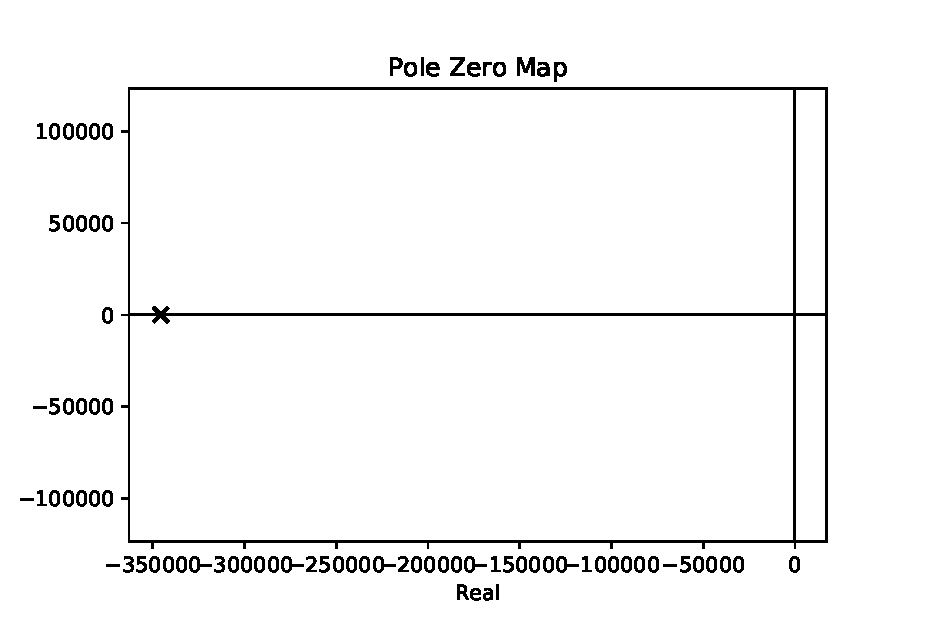
\includegraphics[width=\columnwidth]{./figs/ee18btech11036/ee18btech11036_1.eps}
%\caption{}
%\label{fig:ee18btech11036_ee18btech11036_1}
%\end{figure}
%From  the above graph is is evident that the system has two coinciding poles at frequency 


\item Find $T(0)$ and $\abs{T(\j\omega_p)}$.
\\
%What is the low-frequency gain corresponding  to  the  situation  in  (a)?  What  is  the  valueof the closed-loop gain at the frequency of the coincident poles?\\
\solution From \ref{eq:ee18btech11036_Transfer_func_1}, 
%Putting s=0 in equation 
\begin{align}
    T(0)&= \frac{1000}{3.025} =  50.378 \, dB
    \label{eq:ee18btech11036_zero_gain_value}
\\
\abs{T(\j\omega_p)} &=44.3866
\end{align}
%Plot the transfer function above using the given code  
%\begin{lstlisting}
%codes/ee18btech11036/ee18btech11036_2.py
%\end{lstlisting}
%\begin{figure}[!ht]
%\centering
%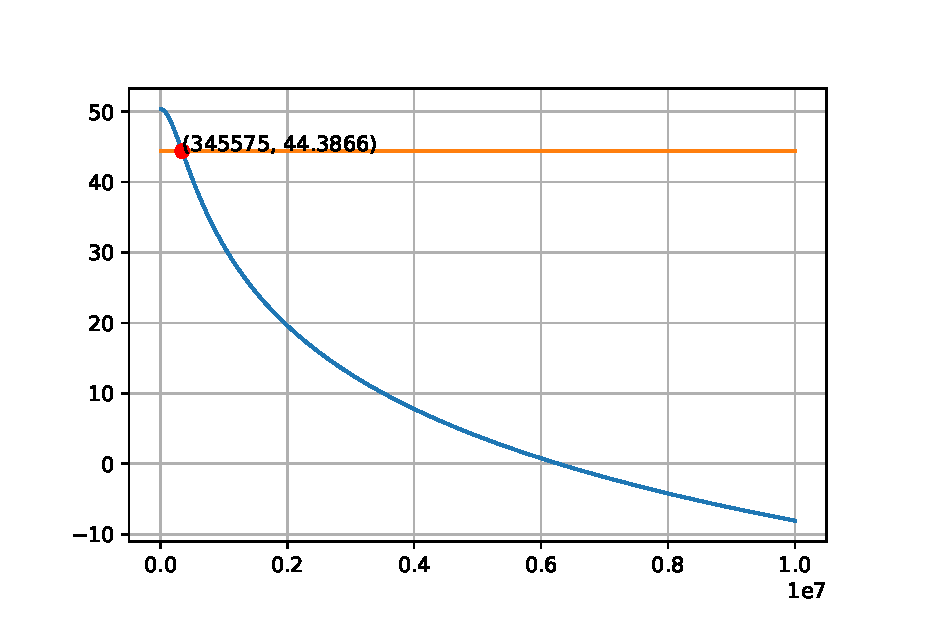
\includegraphics[width=\columnwidth]{./figs/ee18btech11036/ee18btech11036_2.eps}
%\caption{}
%\label{fig:ee18btech11036_ee18btech11036_2}
%\end{figure}
%
%From the plot , the gain (dB) at pole frequency is 44.3866

\item Find $Q$ from      \eqref{eq:ee18btech11036_closed_loop}.
\\
\solution  If the denominator of \eqref{eq:ee18btech11036_closed_loop} is expressed as
%
\begin{multline}
\frac{s^2}{p_1p_2} + \brak{\frac{1}{p_1}+\frac{1}{p_2}}s + HG_0+1 
\\
= s^2+2\zeta\omega_ns+\omega_n^{2} \label{eq:ee18btech11036_second_order_ce}
\end{multline}
then 
%The quality factor Q of equation.\ref{eq:ee18btech11036_second_order_ce}, is given by
\begin{align}
    \omega_n &= {\sqrt{\brak{HG_0+1}p_1p_2}}\\
    \zeta &= {\frac{2p_1p_2}{\sqrt{\brak{HG_0+1}p_1p_2}}}
\end{align}
and 
\begin{align}
    Q &= \frac{1}{2\zeta}
%\end{align}
%
%From equation.\ref{eq:ee18btech11036_closed_loop} and \ref{eq:ee18btech11036_p_values}
%Therefore,For the given second order amplifier with characteristic equation.\ref{eq:ee18btech11036_ce},the Q factor is,
%\begin{align}
\\
     &= \pm{\frac{\sqrt{\brak{1+HG_0}p_1p_2}}{p_1+p_2}} \label{eq:ee18btech11036_Q}
%\end{align}
%From equations \ref{eq:ee18btech11036_h_value} , \ref{eq:ee18btech11036_p_values}
%\begin{align}
\\
     &= 0.5
\end{align}
%---------------------
\item If  H  is  increased  by  a  factor  of  10,  what are the new pole locations? What is the corresponding pole Q?\\
\begin{table}[!ht]
\centering

%%%%%%%%%%%%%%%%%%%%%%%%%%%%%%%%%%%%%%%%%%%%%%%%%%%%%%%%%%%%%%%%%%%%%%
%%                                                                  %%
%%  This is the header of a LaTeX2e file exported from Gnumeric.    %%
%%                                                                  %%
%%  This file can be compiled as it stands or included in another   %%
%%  LaTeX document. The table is based on the longtable package so  %%
%%  the longtable options (headers, footers...) can be set in the   %%
%%  preamble section below (see PRAMBLE).                           %%
%%                                                                  %%
%%  To include the file in another, the following two lines must be %%
%%  in the including file:                                          %%
%%        \def\inputGnumericTable{}                                 %%
%%  at the beginning of the file and:                               %%
%%        \input{name-of-this-file.tex}                             %%
%%  where the table is to be placed. Note also that the including   %%
%%  file must use the following packages for the table to be        %%
%%  rendered correctly:                                             %%
%%    \usepackage[latin1]{inputenc}                                 %%
%%    \usepackage{color}                                            %%
%%    \usepackage{array}                                            %%
%%    \usepackage{longtable}                                        %%
%%    \usepackage{calc}                                             %%
%%    \usepackage{multirow}                                         %%
%%    \usepackage{hhline}                                           %%
%%    \usepackage{ifthen}                                           %%
%%  optionally (for landscape tables embedded in another document): %%
%%    \usepackage{lscape}                                           %%
%%                                                                  %%
%%%%%%%%%%%%%%%%%%%%%%%%%%%%%%%%%%%%%%%%%%%%%%%%%%%%%%%%%%%%%%%%%%%%%%



%%  This section checks if we are begin input into another file or  %%
%%  the file will be compiled alone. First use a macro taken from   %%
%%  the TeXbook ex 7.7 (suggestion of Han-Wen Nienhuys).            %%
\def\ifundefined#1{\expandafter\ifx\csname#1\endcsname\relax}


%%  Check for the \def token for inputed files. If it is not        %%
%%  defined, the file will be processed as a standalone and the     %%
%%  preamble will be used.                                          %%
\ifundefined{inputGnumericTable}

%%  We must be able to close or not the document at the end.        %%
	\def\gnumericTableEnd{\end{document}}


%%%%%%%%%%%%%%%%%%%%%%%%%%%%%%%%%%%%%%%%%%%%%%%%%%%%%%%%%%%%%%%%%%%%%%
%%                                                                  %%
%%  This is the PREAMBLE. Change these values to get the right      %%
%%  paper size and other niceties.                                  %%
%%                                                                  %%
%%%%%%%%%%%%%%%%%%%%%%%%%%%%%%%%%%%%%%%%%%%%%%%%%%%%%%%%%%%%%%%%%%%%%%

	\documentclass[12pt%
			  %,landscape%
                    ]{report}
       \usepackage[latin1]{inputenc}
       \usepackage{fullpage}
       \usepackage{color}
       \usepackage{array}
       \usepackage{longtable}
       \usepackage{calc}
       \usepackage{multirow}
       \usepackage{hhline}
       \usepackage{ifthen}



%%  End of the preamble for the standalone. The next section is for %%
%%  documents which are included into other LaTeX2e files.          %%
\else

%%  We are not a stand alone document. For a regular table, we will %%
%%  have no preamble and only define the closing to mean nothing.   %%
    \def\gnumericTableEnd{}

%%  If we want landscape mode in an embedded document, comment out  %%
%%  the line above and uncomment the two below. The table will      %%
%%  begin on a new page and run in landscape mode.                  %%
%       \def\gnumericTableEnd{\end{landscape}}
%       \begin{landscape}


%%  End of the else clause for this file being \input.              %%
\fi

%%%%%%%%%%%%%%%%%%%%%%%%%%%%%%%%%%%%%%%%%%%%%%%%%%%%%%%%%%%%%%%%%%%%%%
%%                                                                  %%
%%  The rest is the gnumeric table, except for the closing          %%
%%  statement. Changes below will alter the table's appearance.     %%
%%                                                                  %%
%%%%%%%%%%%%%%%%%%%%%%%%%%%%%%%%%%%%%%%%%%%%%%%%%%%%%%%%%%%%%%%%%%%%%%

\providecommand{\gnumericmathit}[1]{#1} 
%%  Uncomment the next line if you would like your numbers to be in %%
%%  italics if they are italizised in the gnumeric table.           %%
%\renewcommand{\gnumericmathit}[1]{\mathit{#1}}
\providecommand{\gnumericPB}[1]%
{\let\gnumericTemp=\\#1\let\\=\gnumericTemp\hspace{0pt}}
 \ifundefined{gnumericTableWidthDefined}
        \newlength{\gnumericTableWidth}
        \newlength{\gnumericTableWidthComplete}
        \newlength{\gnumericMultiRowLength}
        \global\def\gnumericTableWidthDefined{}
 \fi
%% The following setting protects this code from babel shorthands.  %%
 \ifthenelse{\isundefined{\languageshorthands}}{}{\languageshorthands{english}}
%%  The default table format retains the relative column widths of  %%
%%  gnumeric. They can easily be changed to c, r or l. In that case %%
%%  you may want to comment out the next line and uncomment the one %%
%%  thereafter                                                      %%
\providecommand\gnumbox{\makebox[0pt]}
%%\providecommand\gnumbox[1][]{\makebox}

%% to adjust positions in multirow situations                       %%
\setlength{\bigstrutjot}{\jot}
\setlength{\extrarowheight}{\doublerulesep}

%%  The \setlongtables command keeps column widths the same across  %%
%%  pages. Simply comment out next line for varying column widths.  %%
\setlongtables

\setlength\gnumericTableWidth{%
	53pt+%
	93pt+%
0pt}
\def\gumericNumCols{2}
\setlength\gnumericTableWidthComplete{\gnumericTableWidth+%
         \tabcolsep*\gumericNumCols*2+\arrayrulewidth*\gumericNumCols}
\ifthenelse{\lengthtest{\gnumericTableWidthComplete > \linewidth}}%
         {\def\gnumericScale{\ratio{\linewidth-%
                        \tabcolsep*\gumericNumCols*2-%
                        \arrayrulewidth*\gumericNumCols}%
{\gnumericTableWidth}}}%
{\def\gnumericScale{1}}

%%%%%%%%%%%%%%%%%%%%%%%%%%%%%%%%%%%%%%%%%%%%%%%%%%%%%%%%%%%%%%%%%%%%%%
%%                                                                  %%
%% The following are the widths of the various columns. We are      %%
%% defining them here because then they are easier to change.       %%
%% Depending on the cell formats we may use them more than once.    %%
%%                                                                  %%
%%%%%%%%%%%%%%%%%%%%%%%%%%%%%%%%%%%%%%%%%%%%%%%%%%%%%%%%%%%%%%%%%%%%%%

\ifthenelse{\isundefined{\gnumericColA}}{\newlength{\gnumericColA}}{}\settowidth{\gnumericColA}{\begin{tabular}{@{}p{70pt*\gnumericScale}@{}}x\end{tabular}}
\ifthenelse{\isundefined{\gnumericColB}}{\newlength{\gnumericColB}}{}\settowidth{\gnumericColB}{\begin{tabular}{@{}p{45pt*\gnumericScale}@{}}x\end{tabular}}

\begin{tabular}[c]{%
	b{\gnumericColA}%
	b{\gnumericColB}%
	}

%%%%%%%%%%%%%%%%%%%%%%%%%%%%%%%%%%%%%%%%%%%%%%%%%%%%%%%%%%%%%%%%%%%%%%
%%  The longtable options. (Caption, headers... see Goosens, p.124) %%
%	\caption{The Table Caption.}             \\	%
% \hline	% Across the top of the table.
%%  The rest of these options are table rows which are placed on    %%
%%  the first, last or every page. Use \multicolumn if you want.    %%

%%  Header for the first page.                                      %%
%	\multicolumn{2}{c}{The First Header} \\ \hline 
%	\multicolumn{1}{c}{colTag}	%Column 1
%	&\multicolumn{1}{c}{colTag}	\\ \hline %Last column
%	\endfirsthead

%%  The running header definition.                                  %%
%	\hline
%	\multicolumn{2}{l}{\ldots\small\slshape continued} \\ \hline
%	\multicolumn{1}{c}{colTag}	%Column 1
%	&\multicolumn{1}{c}{colTag}	\\ \hline %Last column
%	\endhead

%%  The running footer definition.                                  %%
%	\hline
%	\multicolumn{2}{r}{\small\slshape continued\ldots} \\
%	\endfoot

%%  The ending footer definition.                                   %%
%	\multicolumn{2}{c}{That's all folks} \\ \hline 
%	\endlastfoot
%%%%%%%%%%%%%%%%%%%%%%%%%%%%%%%%%%%%%%%%%%%%%%%%%%%%%%%%%%%%%%%%%%%%%%

\hhline{|-|-}
	 \multicolumn{1}{|p{\gnumericColA}|}%
	{\gnumericPB{\centering}\gnumbox{\textbf{Parameter}}}
	&\multicolumn{1}{p{\gnumericColB}|}%
	{\gnumericPB{\centering}\gnumbox{\textbf{Value}}}
\\
\hhline{|-|-}
	 \multicolumn{1}{|p{\gnumericColA}|}%
	{\gnumericPB{\centering}\gnumbox{\text{H}}}
	&\multicolumn{1}{p{\gnumericColB}|}%
	{\gnumericPB{\centering}\gnumbox{\text{0.002025}}}
\\
\hhline{|-|-}
	 \multicolumn{1}{|p{\gnumericColA}|}%
	{\gnumericPB{\centering}\gnumbox{\text{Gain (0 freq)}}}
	&\multicolumn{1}{p{\gnumericColB}|}%
	{\gnumericPB{\centering}\gnumbox{\text{50.378}}}
\\
\hhline{|-|-}
	 \multicolumn{1}{|p{\gnumericColA}|}%
	{\gnumericPB{\centering}\gnumbox{\text{Gain (pole freq)}}}
	&\multicolumn{1}{p{\gnumericColB}|}%
	{\gnumericPB{\centering}\gnumbox{\text{44.38}}}
\\
\hhline{|-|-}
	 \multicolumn{1}{|p{\gnumericColA}|}%
	{\gnumericPB{\centering}\gnumbox{\text{Q}}}
	&\multicolumn{1}{p{\gnumericColB}|}%
	{\gnumericPB{\centering}\gnumbox{\text{0.5}}}
\\


\hhline{|-|-|}
\end{tabular}

\ifthenelse{\isundefined{\languageshorthands}}{}{\languageshorthands{\languagename}}
\gnumericTableEnd

\caption{}
\label{table:ee18btech11036_ out_Table}
\end{table}

\solution  From     \eqref{eq:ee18btech11036_h_value},

%H is increased by factor of 10, hence
\begin{align}
     H=0.02025
     \label{eq:ee18btech11036_new_h}
\end{align}
which, upon substitution in  \ref{eq:ee18btech11036_closed_loop} yields
%
\begin{align}
    T(s) &= \frac{1000}{2.533 \times 10^{-11}s^2+1.750 \times 10^{-5}s+21.25}
    \label{eq:ee18btech11036_Transfer_func_2}
\end{align}
The new pole locations are given by the following code
\begin{lstlisting}
codes/ee18btech11036/ee18btech11036_3.py
\end{lstlisting}

%\begin{figure}[!ht]
%\centering
%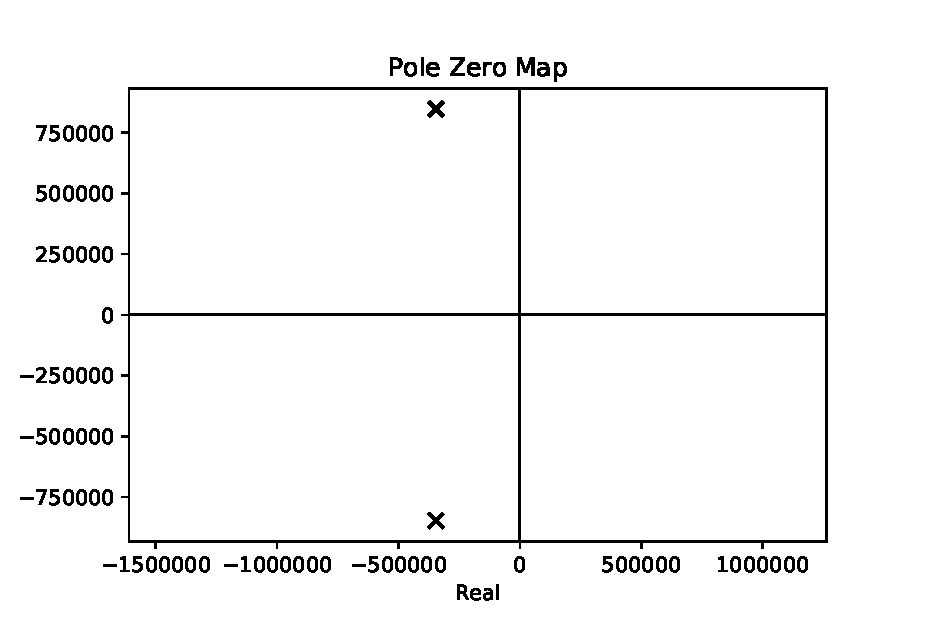
\includegraphics[width=\columnwidth]{./figs/ee18btech11036/ee18btech11036_3.eps}
%\caption{}
%\label{fig:ee18btech11036_ee18btech11036_3}
%\end{figure}
%Poles are : 
% \begin{align}
%     $p_1$ &= -345575.19 + j848230.0    
% \\
%     $p_2$ &= -345575.19 - j848230.0
% %     \label{eq:ee18btech11036_new_poles}
% \end{align}

%From equation \ref{eq:ee18btech11036_Q}
%\begin{align}
%    Q &= \pm{\frac{\sqrt{\brak{1+10HG_0}p_1p_2}}{p_1+p_2}} \label{eq:ee18btech11036_Q_2}
%\end{align}
%Solving this we get :
%
and 
\begin{align}
    Q=1.325
    \label{eq:ee18btech11036_Q_new2}
\end{align}
%-----------------

\item Find the step response of $T(s)$
\\
\solution The following code generates the desired response  in Fig. \ref{fig:ee18btech11036_ee18btech11036_4}.
\begin{lstlisting}
codes/ee18btech11036/ee18btech11036_4.py
\end{lstlisting}
%
\begin{figure}[!ht]
\centering
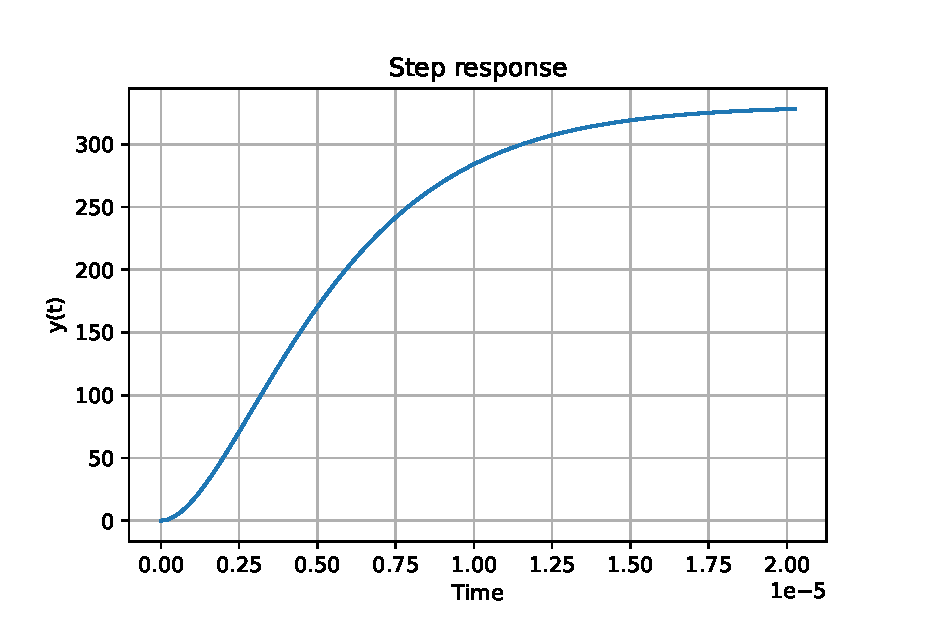
\includegraphics[width=\columnwidth]{./figs/ee18btech11036/ee18btech11036_4.eps}
\caption{}
\label{fig:ee18btech11036_ee18btech11036_4}
\end{figure}



%-------------------------------
\item Design a circuit for $T(s)$ in \eqref{eq:ee18btech11036_Transfer_func_1}.
\\
\numberwithin{figure}{enumi}
\solution Consider the circuit in 
%The circuit can be designed using an operational amplifiers having negative feedback.Consider the circuit shown in 
Fig. \ref{fig:ee18btech11036_equivalent_control_system}.
%:1.Assume the gain of all the amplifiers are large.And assume no zero state response.Take the parameters in s-domain.\\
\renewcommand{\thefigure}{\theenumi.\arabic{figure}}
\begin{figure}[!hbt]
	\begin{center}
			\resizebox{\columnwidth}{!}{ \begin{circuitikz}
\ctikzset{bipoles/length=1cm}

\draw 
   (0, 0) node[op amp] (opamp) {}
    (4.5, -0.35) node[op amp] (opamp2) {}
    (9, -0.7) node[op amp] (opamp3) {}
    (opamp.-) -- (-1,0.35) -- (-1.5,0.35) to[R=$R_3$] (-3,0.35){}
    (-1,0.35)-- (-1,1) to[R=$R_4$] (1.5,1) -- (1.5,0){}
    (opamp.+) -- (-1,-0.35) to[R=$R_1$] (-3,-0.35){}
    (opamp.out)--(1.5,0){}
    (-1,-0.35) to[R=$R_2$] (-1,-1.5) node[ground]{}
   
    (1.5,0)--(2,0) to[R=$R_5$] (3,0)--(3.5,0)--(opamp2.-){}
    (3.5,0.75)--(3.5,1.5) to[C=$C_1$] (6,1.5)--(6,0.35){}
    (3.5,0) -- (3.5,0.75)--(4,0.75) to[R=$R_6$] (6,0.75) -- (6,-0.35){}
    (opamp2.+)--(3.5,-0.7) node[ground]{}
    (opamp2.out) -- (6,-0.35){}
    (6,-0.35)--(6.5,-0.35) to[R=$R_7$] (7.5,-0.35)--(8,-0.35)--(opamp3.-){}
    (opamp3.+)--(8,-1.05) node[ground]{}
    (8,-0.35) -- (8,0.75) to[R=$R_8$] (10,0.75) -- (10,-0.7){}
    (8,0.75)--(8,1.5) to[C=$C_2$] (10,1.5)--(10,0.35){}
    (10,1.5)--(10,4) to[R=$R_9$] (-3,4)--(-3,0.35){}
    (opamp3.out) -- (11,-0.7){}
    (2,4) to[R=$R_{10}$] (2,3) node[ground]{}

    node at (-1,-0.3){$V_p$}
    node at (-1,0.3){$V_e$}
    node at (3.5,-0.2){$V_a$}
    node at (8,-0.6) {$V_b$}
    % node at (12,-1){D}

    node at (1.5,-0.4){$V_1$}
    node at (6,-0.6){$V_2$}

    node at (11,-1) {$V_{out}$}
    node at(-3.5,-0.35){$V_{in}$}
    node at(-3.5,0.27){$V_{f}$}

;\end{circuitikz}



}
	\end{center}
\caption{}
\label{fig:ee18btech11036_equivalent_control_system}
\end{figure}
%
%Then
%%\textbf{For the first amplifier..,}
%%Applying KCL at node A., 
%%Since, the opamp has large gain, potential at node A is assumed to be zero due to virtual short at node A.
%\begin{align}
%%    \frac{0-V_{in}(s)}{R_1} +\frac{0-V_1(s)}{R_2} &= 0\\
%%    \frac{V_{in}(s)}{R_1} &= \frac{V_1(s)}{R_2}\\
%%\implies 
%V_{in} &= -\frac{V_1(s) R_1}{R_2}\label{eq:ee18btech11036_opamp_1}
%%\end{align}
%%\textbf{For the second amplifier..,}
%%Applying KCL at node B..,
%%Similarly potential at node B is zero.
%%\begin{align}
%%  \frac{-V_1(s)}{R}+\frac{-V_2(s)}{R}-sCV_2(s)+\frac{-V_{out}(s)}{R} &= 0\\
%%  \frac{-V_1(s)}{R}+\frac{-V_2(s)}{R}-sCV_2(s) = \frac{V_{out}(s)}{R} \\
%\\
%  \frac{-V_1(s)}{R} &= V_2(s)\sbrak{sC+\frac{1}{R}}+\frac{V{out}(s)}{R} \label{eq:ee18btech11036_opamp_2}
%%\end{align}
%%\textbf{For the third amplifier..,}
%%Potential at node C is zero(Due to high gain of amplifier).Applying KCL at node C.
%%\begin{align}
%%    \frac{-V_2(s)}{R}+\frac{-V_3(s)}{R} = 0\\
%%    \implies 
%\\
%V_2(s) &= -V_3(s) \label{eq:ee18btech11036_opamp_3}
%%\end{align}
%%\textbf{For the Fourth amplifier.,}
%%Potential at node D is zero.Applying KCL at node D.
%%\begin{align}
%%    \frac{-V_3(s)}{R}+sC_1(-V_{out}(s)) = 0\\
%\\
%    V_3(s) &= -sC_1RV_{out}(s) \label{eq:ee18btech11036_opamp_4}
%\end{align}
%by computing the closed loop gain for each opamp.
%From equation.\ref{eq:ee18btech11036_opamp_4} and equation. \ref{eq:ee18btech11036_opamp_3}..,
%\begin{align}
%    V_2(s) = sC_1RV_{out}(s) \label{eq:ee18btech11036_eq_1}
%\end{align}
%Substituting the equation.\ref{eq:ee18btech11036_opamp_2} and equation.\ref{eq:ee18btech11036_eq_1},
%\begin{align}
%    \frac{-V_1(s)}{R} &= \brak{s^2C_1CR + sC_1}V_{out}(s) +\frac{V_{out}(s)}{R}\\
%    V_1(s) &= -\brak{s^2C_1CR^2+sC_1R+1}V_{out}(s)\label{eq:ee18btech11036_eq_2}
%\end{align}
%from equation.\ref{eq:ee18btech11036_opamp_1} and equation.\ref{eq:ee18btech11036_eq_2}.
\begin{align}
%     V_1(s) &= \frac{R_1}{R_2}\brak{s^2C_1CR^2+sC_1R+1}V_{out}(s)\\
    \frac{V_{out}(s)}{V_{in}(s)} &= \frac{R_2}{R_1\brak{s^2C_1CR^2+sC_1R+1}} 
    \label{eq:ee18btech11036_eq_3}
\end{align}
Using parameters from \ref{table:ee18btech11036_ Output_Table} in 
\eqref{eq:ee18btech11036_eq_3}, \eqref{eq:ee18btech11036_Transfer_func_1} is obtained.
%Comparing equation.\ref{eq:ee18btech11036_Transfer_func_1} and equation.\ref{eq:ee18btech11036_eq_3}
%\begin{align}
%    R_2 &= 33k\Omega \\
%    R_1 &= 100 \Omega\\
%    C_1CR^2 &= 0.8373x10^{-11} \\
%    C_1R &= 0.5785x10^{-5} F\\
%\text{Let.,} C_1 &= 4 nF \\
%\implies C &= 1 nF \\
% \text{and.,} C_1R &= 0.5785x10^{-5} F \\
% \implies R &= 1.446 k\Omega
%\end{align}

\begin{table}[!ht]
\centering

%%%%%%%%%%%%%%%%%%%%%%%%%%%%%%%%%%%%%%%%%%%%%%%%%%%%%%%%%%%%%%%%%%%%%%
%%                                                                  %%
%%  This is the header of a LaTeX2e file exported from Gnumeric.    %%
%%                                                                  %%
%%  This file can be compiled as it stands or included in another   %%
%%  LaTeX document. The table is based on the longtable package so  %%
%%  the longtable options (headers, footers...) can be set in the   %%
%%  preamble section below (see PRAMBLE).                           %%
%%                                                                  %%
%%  To include the file in another, the following two lines must be %%
%%  in the including file:                                          %%
%%        \def\inputGnumericTable{}                                 %%
%%  at the beginning of the file and:                               %%
%%        \input{name-of-this-file.tex}                             %%
%%  where the table is to be placed. Note also that the including   %%
%%  file must use the following packages for the table to be        %%
%%  rendered correctly:                                             %%
%%    \usepackage[latin1]{inputenc}                                 %%
%%    \usepackage{color}                                            %%
%%    \usepackage{array}                                            %%
%%    \usepackage{longtable}                                        %%
%%    \usepackage{calc}                                             %%
%%    \usepackage{multirow}                                         %%
%%    \usepackage{hhline}                                           %%
%%    \usepackage{ifthen}                                           %%
%%  optionally (for landscape tables embedded in another document): %%
%%    \usepackage{lscape}                                           %%
%%                                                                  %%
%%%%%%%%%%%%%%%%%%%%%%%%%%%%%%%%%%%%%%%%%%%%%%%%%%%%%%%%%%%%%%%%%%%%%%



%%  This section checks if we are begin input into another file or  %%
%%  the file will be compiled alone. First use a macro taken from   %%
%%  the TeXbook ex 7.7 (suggestion of Han-Wen Nienhuys).            %%
\def\ifundefined#1{\expandafter\ifx\csname#1\endcsname\relax}


%%  Check for the \def token for inputed files. If it is not        %%
%%  defined, the file will be processed as a standalone and the     %%
%%  preamble will be used.                                          %%
\ifundefined{inputGnumericTable}

%%  We must be able to close or not the document at the end.        %%
	\def\gnumericTableEnd{\end{document}}


%%%%%%%%%%%%%%%%%%%%%%%%%%%%%%%%%%%%%%%%%%%%%%%%%%%%%%%%%%%%%%%%%%%%%%
%%                                                                  %%
%%  This is the PREAMBLE. Change these values to get the right      %%
%%  paper size and other niceties.                                  %%
%%                                                                  %%
%%%%%%%%%%%%%%%%%%%%%%%%%%%%%%%%%%%%%%%%%%%%%%%%%%%%%%%%%%%%%%%%%%%%%%

	\documentclass[12pt%
			  %,landscape%
                    ]{report}
       \usepackage[latin1]{inputenc}
       \usepackage{fullpage}
       \usepackage{color}
       \usepackage{array}
       \usepackage{longtable}
       \usepackage{calc}
       \usepackage{multirow}
       \usepackage{hhline}
       \usepackage{ifthen}



%%  End of the preamble for the standalone. The next section is for %%
%%  documents which are included into other LaTeX2e files.          %%
\else

%%  We are not a stand alone document. For a regular table, we will %%
%%  have no preamble and only define the closing to mean nothing.   %%
    \def\gnumericTableEnd{}

%%  If we want landscape mode in an embedded document, comment out  %%
%%  the line above and uncomment the two below. The table will      %%
%%  begin on a new page and run in landscape mode.                  %%
%       \def\gnumericTableEnd{\end{landscape}}
%       \begin{landscape}


%%  End of the else clause for this file being \input.              %%
\fi

%%%%%%%%%%%%%%%%%%%%%%%%%%%%%%%%%%%%%%%%%%%%%%%%%%%%%%%%%%%%%%%%%%%%%%
%%                                                                  %%
%%  The rest is the gnumeric table, except for the closing          %%
%%  statement. Changes below will alter the table's appearance.     %%
%%                                                                  %%
%%%%%%%%%%%%%%%%%%%%%%%%%%%%%%%%%%%%%%%%%%%%%%%%%%%%%%%%%%%%%%%%%%%%%%

\providecommand{\gnumericmathit}[1]{#1} 
%%  Uncomment the next line if you would like your numbers to be in %%
%%  italics if they are italizised in the gnumeric table.           %%
%\renewcommand{\gnumericmathit}[1]{\mathit{#1}}
\providecommand{\gnumericPB}[1]%
{\let\gnumericTemp=\\#1\let\\=\gnumericTemp\hspace{0pt}}
 \ifundefined{gnumericTableWidthDefined}
        \newlength{\gnumericTableWidth}
        \newlength{\gnumericTableWidthComplete}
        \newlength{\gnumericMultiRowLength}
        \global\def\gnumericTableWidthDefined{}
 \fi
%% The following setting protects this code from babel shorthands.  %%
 \ifthenelse{\isundefined{\languageshorthands}}{}{\languageshorthands{english}}
%%  The default table format retains the relative column widths of  %%
%%  gnumeric. They can easily be changed to c, r or l. In that case %%
%%  you may want to comment out the next line and uncomment the one %%
%%  thereafter                                                      %%
\providecommand\gnumbox{\makebox[0pt]}
%%\providecommand\gnumbox[1][]{\makebox}

%% to adjust positions in multirow situations                       %%
\setlength{\bigstrutjot}{\jot}
\setlength{\extrarowheight}{\doublerulesep}

%%  The \setlongtables command keeps column widths the same across  %%
%%  pages. Simply comment out next line for varying column widths.  %%
\setlongtables

\setlength\gnumericTableWidth{%
	53pt+%
	93pt+%
0pt}
\def\gumericNumCols{2}
\setlength\gnumericTableWidthComplete{\gnumericTableWidth+%
         \tabcolsep*\gumericNumCols*2+\arrayrulewidth*\gumericNumCols}
\ifthenelse{\lengthtest{\gnumericTableWidthComplete > \linewidth}}%
         {\def\gnumericScale{\ratio{\linewidth-%
                        \tabcolsep*\gumericNumCols*2-%
                        \arrayrulewidth*\gumericNumCols}%
{\gnumericTableWidth}}}%
{\def\gnumericScale{1}}

%%%%%%%%%%%%%%%%%%%%%%%%%%%%%%%%%%%%%%%%%%%%%%%%%%%%%%%%%%%%%%%%%%%%%%
%%                                                                  %%
%% The following are the widths of the various columns. We are      %%
%% defining them here because then they are easier to change.       %%
%% Depending on the cell formats we may use them more than once.    %%
%%                                                                  %%
%%%%%%%%%%%%%%%%%%%%%%%%%%%%%%%%%%%%%%%%%%%%%%%%%%%%%%%%%%%%%%%%%%%%%%

\ifthenelse{\isundefined{\gnumericColA}}{\newlength{\gnumericColA}}{}\settowidth{\gnumericColA}{\begin{tabular}{@{}p{70pt*\gnumericScale}@{}}x\end{tabular}}
\ifthenelse{\isundefined{\gnumericColB}}{\newlength{\gnumericColB}}{}\settowidth{\gnumericColB}{\begin{tabular}{@{}p{45pt*\gnumericScale}@{}}x\end{tabular}}

\begin{tabular}[c]{%
	b{\gnumericColA}%
	b{\gnumericColB}%
	}

%%%%%%%%%%%%%%%%%%%%%%%%%%%%%%%%%%%%%%%%%%%%%%%%%%%%%%%%%%%%%%%%%%%%%%
%%  The longtable options. (Caption, headers... see Goosens, p.124) %%
%	\caption{The Table Caption.}             \\	%
% \hline	% Across the top of the table.
%%  The rest of these options are table rows which are placed on    %%
%%  the first, last or every page. Use \multicolumn if you want.    %%

%%  Header for the first page.                                      %%
%	\multicolumn{2}{c}{The First Header} \\ \hline 
%	\multicolumn{1}{c}{colTag}	%Column 1
%	&\multicolumn{1}{c}{colTag}	\\ \hline %Last column
%	\endfirsthead

%%  The running header definition.                                  %%
%	\hline
%	\multicolumn{2}{l}{\ldots\small\slshape continued} \\ \hline
%	\multicolumn{1}{c}{colTag}	%Column 1
%	&\multicolumn{1}{c}{colTag}	\\ \hline %Last column
%	\endhead

%%  The running footer definition.                                  %%
%	\hline
%	\multicolumn{2}{r}{\small\slshape continued\ldots} \\
%	\endfoot

%%  The ending footer definition.                                   %%
%	\multicolumn{2}{c}{That's all folks} \\ \hline 
%	\endlastfoot
%%%%%%%%%%%%%%%%%%%%%%%%%%%%%%%%%%%%%%%%%%%%%%%%%%%%%%%%%%%%%%%%%%%%%%

\hhline{|-|-}
	 \multicolumn{1}{|p{\gnumericColA}|}%
	{\gnumericPB{\centering}\gnumbox{\textbf{Parameter}}}
	&\multicolumn{1}{p{\gnumericColB}|}%
	{\gnumericPB{\centering}\gnumbox{\textbf{Value}}}
\\
\hhline{|-|-}
	 \multicolumn{1}{|p{\gnumericColA}|}%
	{\gnumericPB{\centering}\gnumbox{\text{$R_1$}}}
	&\multicolumn{1}{p{\gnumericColB}|}%
	{\gnumericPB{\centering}\gnumbox{\text{100 $\Omega$}}}
\\
\hhline{|-|-}
	 \multicolumn{1}{|p{\gnumericColA}|}%
	{\gnumericPB{\centering}\gnumbox{\text{$R_2$}}}
	&\multicolumn{1}{p{\gnumericColB}|}%
	{\gnumericPB{\centering}\gnumbox{\text{33 k$\Omega$}}}
\\
\hhline{|-|-}
	 \multicolumn{1}{|p{\gnumericColA}|}%
	{\gnumericPB{\centering}\gnumbox{\text{R}}}
	&\multicolumn{1}{p{\gnumericColB}|}%
	{\gnumericPB{\centering}\gnumbox{\text{1.446 k$\Omega$}}}
\\
\hhline{|-|-}
	 \multicolumn{1}{|p{\gnumericColA}|}%
	{\gnumericPB{\centering}\gnumbox{\text{C}}}
	&\multicolumn{1}{p{\gnumericColB}|}%
	{\gnumericPB{\centering}\gnumbox{\text{1 nF}}}
\\
\hhline{|-|-}
	 \multicolumn{1}{|p{\gnumericColA}|}%
	{\gnumericPB{\centering}\gnumbox{\text{$C_1$}}}
	&\multicolumn{1}{p{\gnumericColB}|}%
	{\gnumericPB{\centering}\gnumbox{\text{4 nF}}}
\\

\hhline{|-|-|}
\end{tabular}

\ifthenelse{\isundefined{\languageshorthands}}{}{\languageshorthands{\languagename}}
\gnumericTableEnd

\caption{}
\label{table:ee18btech11036_ Output_Table}
\end{table}
 The circuit can be represented as block diagram as shown in Fig. \ref{fig:ee18btech11036_block_diag}
\begin{figure}[!hbt]
	\begin{center}
			\resizebox{\columnwidth}{!}{\tikzstyle{block} = [draw, rectangle, 
    minimum height=1.25em, minimum width=2.5em]
\tikzstyle{sum} = [draw, circle, node distance=1cm]
\tikzstyle{input} = [coordinate]
\tikzstyle{output} = [coordinate]
\tikzstyle{pinstyle} = [pin edge={to-,thin,black}]

% The block diagram code is probably more verbose than necessary
\begin{tikzpicture}[auto, node distance=4cm,>=latex']
    % We start by placing the blocks
    \node [input, name=input] {};
    \node [sum, right of=input] (sum) {};
    \node [block, right of=sum] (g1) {$\frac{-R_6}{(R_5)(1+sC_1R_6)}$};
    \node [block, right of=g1] (g2) {$\frac{-R_8}{(R_7)(1+sC_2R_8)}$};
    \node [output, right of=g2] (output) {};
    \node [block, below of=g2] (feedback_gain) {$\frac{R_{10}}{R_9+R_{10}}$};
    % \node [block, right of=controller, pin={[pinstyle]above:Disturbances},
    %         node distance=3cm] (system) {System};
    % We draw an edge between the controller and system block to 
    % calculate the coordinate u. We need it to place the measurement block. 
    %\draw [->] (controller) -- node[name=u] {$u$} (system);
    % \node [output, right of=system] (output) {};
    % \node [block, below of=u] (measurements) {Measurements};
    % \draw [draw,->] (input) -- node[pos=0.99] {$+$} node {$V_{s}$} (gain);
    % % Once the nodes are placed, connecting them is easy. 
    % % \draw [draw,->] (input) -- node {$r$} ();
    % \draw [->] (gain) -- node {$e$} (sum);
    % \draw [->] (system) -- node [name=y] {$y$}(output);
    % \draw [->] (y) |- (measurements);
    % \draw [->] (measurements) -| node[pos=0.99] {$-$} 
    %     node [near end] {$y_m$} (sum);
    \draw [draw,->] (input) -- node[pos=0.99] {$ $} node {$V_{in}$} (sum);
    \draw [->] (sum) -- node {$ $} (g1);
    \draw [->] (g1) -- node {$  $} (g2);
    \draw [->] (g2) -- node [name=y] {$V_{o}$}(output);
    \draw [->] (y) |- (feedback_gain);
    \draw [->] (feedback_gain) -| node[pos=0.99] {$-$} node [near end] {$V_{f}$} (sum);
\end{tikzpicture}}
	\end{center}
\caption{}
\label{fig:ee18btech11036_block_diag}
\end{figure}
\renewcommand{\thefigure}{\theenumi}
\\
Solving this block diagram:
\begin{align}
%     V_1(s) &= \frac{R_1}{R_2}\brak{s^2C_1CR^2+sC_1R+1}V_{out}(s)\\
    T(s) &= \frac{-R_2}{R_1}\brak{\frac{G(s)}{1+G(s)H(s)}}
    \label{eq:ee18btech11036_eq_5}
    \\
    T(s) &= \frac{-R_2}{R_1}\brak{\frac{\frac{-1}{\brak{1+sCR}\brak{sCR_1}}}{1+\frac{-1}{\brak{1+sCR}\brak{sCR_1}}\brak{-1}}}
    \label{eq:ee18btech11036_eq_6}
    \\
    \implies T(s) &= \frac{R_2}{R_1\brak{s^2C_1CR^2+sC_1R+1}} 
\end{align}
Transfer function was found to be same as given in equation \ref{eq:ee18btech11036_eq_3}

%--------------------------------
\item Verify the step response of the output from ngspice simulation.\\
\solution The following netlist file does the transient anaylsis and store the Vout values with respect to time in a dat file. 
\begin{lstlisting}
codes/ee18btech11036/spice/ngspice_db.net
\end{lstlisting}
Following python code is to plot the step response.
\begin{lstlisting}
codes/ee18btech11036/spice/ee18btech11036_spice.py
\end{lstlisting}
The step response obtained is shown in Fig. \ref{fig:ee18btech11036_ee18btech11036_5}.The graph has steady state value equal to 50.3 dB/330 V.
\begin{figure}[!ht]
\centering
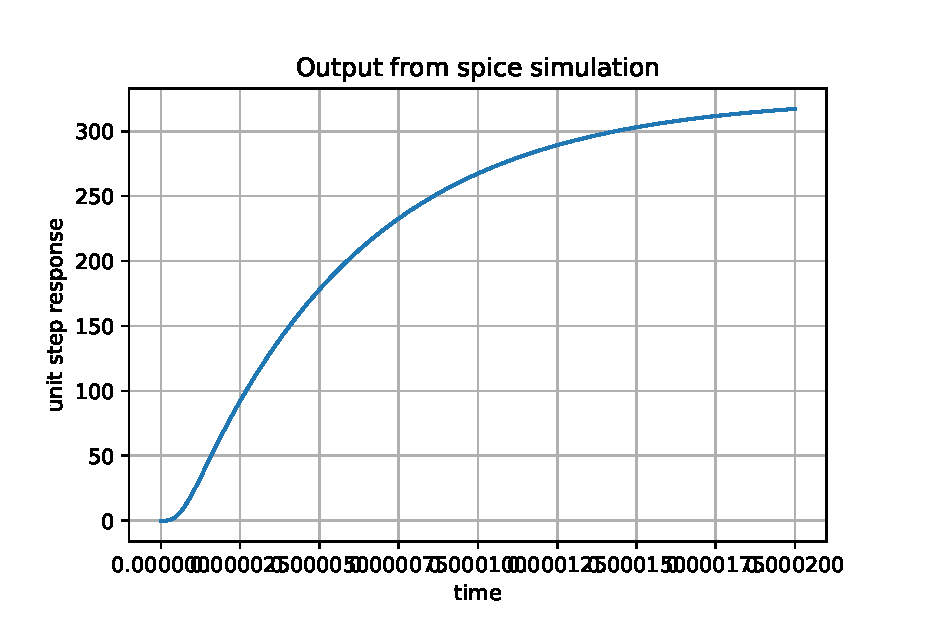
\includegraphics[width=\columnwidth]{./figs/ee18btech11036/ee18btech11036_5.eps}
\caption{}
\label{fig:ee18btech11036_ee18btech11036_5}
\end{figure}

\end{enumerate}




\end{document}
